\documentclass[11pt]{article}
\usepackage[top=2cm,bottom=2cm,left=1.75cm,right= 1.75cm]{geometry}
%\geometry{landscape}                % Activate for for rotated page geometry
\usepackage[parfill]{parskip}    % Activate to begin paragraphs with an empty line rather than an indent
\usepackage{graphicx}
\usepackage{amssymb}
\usepackage{epstopdf}
\usepackage{amsmath}
\usepackage{multirow}
\usepackage{hyperref}
%\usepackage{changepage}
\usepackage{lscape}
%\usepackage{ulem}
\usepackage{multicol}
\usepackage{setspace}
\usepackage{dashrule}
\usepackage[usenames,dvipsnames]{color}
\usepackage{enumerate}
\usepackage{enumitem}
\newcommand{\urlwofont}[1]{\urlstyle{same}\url{#1}}
\newcommand{\degree}{\ensuremath{^\circ}}
\newcommand{\hl}[1]{\textbf{\underline{#1}}}
\newcommand\given[1][]{\:#1\vert\:}

% footnote citation
\usepackage[style=authortitle-ibid, maxnames=3,natbib=true,sortcites=true,block=space]{biblatex}
\bibliography{final}

% color hyperlinks
%\usepackage[colorlinks=false,pdfborder={0 0 0},urlcolor= MidnightBlue,colorlinks=true,linkcolor= MidnightBlue, citecolor= MidnightBlue,backref=true]{hyperref}

\DeclareGraphicsRule{.tif}{png}{.png}{`convert #1 `dirname #1`/`basename #1 .tif`.png}

\newenvironment{choices}{
\begin{enumerate}[(a)]
}{\end{enumerate}}

%\newcommand{\soln}[2]{\textcolor{MidnightBlue}{\textit{#2}}}{} 		% solutions
\newcommand{\soln}[2]{\vspace{#1}}{}						% exam, handout, etc.

%\newcommand{\solnMult}[1]{\textbf{\textcolor{MidnightBlue}{\textit{#1}}}}	% uncomment for solutions
\newcommand{\solnMult}[1]{ #1 }	% uncomment for handouts

%\newcommand{\tf}[1]{ \textbf{\textcolor{MidnightBlue}{\textit{#1}}} }	% uncomment for solutions
\newcommand{\tf}[1]{}	% uncomment for handouts

%\newcommand{\pts}[1]{ \textbf{{\small \textcolor{BurntOrange}{(#1)}}} }	% uncomment for solutions
\newcommand{\pts}[1]{ \textbf{{\small \textcolor{black}{(#1)}}} }	% uncomment for handouts

\newcommand{\note}[1]{ \textbf{\textcolor{red}{[#1]}} }	% uncomment for handouts

\newcommand{\qt}[1]{\textcolor{RoyalBlue}{\textbf{\textit{#1.}}}}

\renewcommand{\emph}[1]{\underline{\textbf{#1}}}

\newcommand{\reference}[1]{ \textbf{\textcolor{red}{[#1]}} }

%\newcommand{\fb}[3]{
%  \textcolor{NavyBlue}{\textbf{Question Feedback:} #1} \\$\:$\\
%  \textcolor{NavyBlue}{\textbf{This question refers to the following learning objective(s):}\\
%  \textbf{\textit{#2:}} #3}
%}


\begin{document}

\begin{titlepage}

\enlargethispage{\baselineskip}


STA 112 \hfill Dr. Evans \\
Spring 2022	\hfill Exam 1\\

\vspace{-2cm}

\begin{center}
{\Huge Exam 1}	
\end{center}

$\:$ \\

\textbf{Last Name:} \rule{5cm}{0.5pt}	\hfill	 \textbf{First Name:}  \rule{5cm}{0.5pt}	 \\
$\:$ \\
%\textbf{Section:} A (11 AM) $\quad$ B (9:30 AM) \hfill	
%\textbf{Team Name:}  \rule{7cm}{0.5pt} \\
$\:$ \\

\textit{I hereby state that I have not communicated with or gained information in any way from other students or any outside resource during this exam. I agree to abide by the rules stated below, and to abide by the Wake Forest Honor Code. All work is my own. I understand that any violation of this agreement will be reported to the Honor Council and will result, at minimum, in a 0 on this exam.}
\[ Signature: \rule{7cm}{0.5pt}\]

\hdashrule[0.5ex]{\textwidth}{0.5pt}{3mm}

\textbf{All work on this exam must be your own.}

{\small
\begin{enumerate}
\item You have 50 minutes to complete the exam.
\item Show all your work on the open ended questions in order to get partial credit. No credit will be given for open ended questions where no work is shown, even if the answer is correct.
\item You are allowed a calculator, however you may not share a calculator with another student during the exam. The calculator must be only a calculator, and may not be connected to the internet. 
\item You are allowed to ask clarification questions to me, but you may not ask anyone else. 
\item You are \hl{not} allowed a cell phone, even if you intend to use it as a calculator or for checking the time. You are \hl{not} allowed a music device or headphones, notes, books, or other resources. 
\item You may \hl{not} communicate with anyone other than myself during the exam.
\item Write clearly and be clear. Make it easy to find your answers. 
\end{enumerate}
}
\begin{center}
{\Large Good luck!}
\end{center}
\hdashrule[0.5ex]{\textwidth}{0.5pt}{3mm}

%\begin{center}
%\includegraphics[width=0.5\textwidth]{../figures/bubbles_new}
%\end{center}



\end{titlepage}

\pagebreak

%%%%%%%%%%%%%%%%%%%%%%%%%%%%%%%%%%%%%%%
$\:$ \\
\thispagestyle{empty}
\pagebreak

%%%%%%%%%%%%%%%%%%%%%%%%%%%%%%%%%%%%%%%
\setcounter{page}{1}
%%%%%%%%%%%%%%%%%%%%%%%%%%%%%%%%%%%%%%%

%\rule{\textwidth}{1pt}
%\begin{center}
%\textit{Answer questions \ref{DriveStart} to \ref{DriveEnd} based on the information %below.} \\
%\end{center}
\rule{\textwidth}{0.5pt}

\textbf{The Data} We have a client who is interested in examining a recent advertising campaign for DoorDash, a popular food service in which food from restaurants is picked up and delivered to your door. The client wants to examine the relationship between exposure to advertising and the use of the service at a local university. They have data on 150 randomly selected students from this university, and the data were collected during the month of September when the campaign was active. 

We have information on X = the amount of exposure a student has to the ad campaign  during the month (measured in minutes, between 0 to 6 minutes. Decimals are permitted for values less than a whole minute) and Y = the amount of money the student spent on DoorDash during that month (in US dollars).

\rule{\textwidth}{1pt}

\begin{enumerate}

\item Based on the information we have so far, write down a population model you would suggest the client consider to model the desired relationship. Use appropriate notation. 



\pagebreak

%%%%%%%%%%%%%%%%%%%%%%%%%%%%%%%%%%%%%%%%

The client fits the model and obtains the following output: 

\textbf{Model 1} 

\begin{center}
\begin{tabular}{rrrrr}
  \hline
             & Estimate & Std. Error \\
  \hline
(Intercept)    & 4.50 & 0.12    \\
 AdExposure    & 1.26 & 0.08 \\
  \hline
\end{tabular}
\end{center}

\rule{\textwidth}{1pt}

\item Based on the output above, write down the equation of the fitted model. 



\vspace{4cm} 


\item Interpret the slope and intercept of the fitted model. 

\vspace{5cm}

\item What is the predicted amount spent by a student who was exposed to 3 minutes of DoorDash ads? Show all your work.


\pagebreak


%%%%%%%%%%%%%%%%%%%%%%%%%%%%%%%%%%


\textbf{Model 1} 

\begin{center}
\begin{tabular}{rrrrr}
  \hline
             & Estimate & Std. Error \\
  \hline
(Intercept)    & 4.50 & 0.12    \\
 AdExposure    & 1.26 & 0.08 \\
  \hline
\end{tabular}
\end{center}

\rule{\textwidth}{1pt}

The client is interested in whether there is a positive relationship between ad exposure and the amount students spend on DoorDash.

\item The client builds a 99\% confidence interval for the slope, and interprets it as follows. ``There is a 99\% probability that the slope 1.26 falls between 1.18 and 1.34.'' (a) Is the client's confidence interval and interpretation correct? (b) If so, show work to back up the client's claim. If not, provide the correct confidence interval and interpretation. For reference, the critical value is $t^* = 2.61$.


\pagebreak

%%%%%%%%%%%%%%%%%%%%%%%%%%%%%%%%%%%%%

\textbf{Model 1} 

\begin{center}
\begin{tabular}{rrrrr}
  \hline
             & Estimate & Std. Error \\
  \hline
(Intercept)    & 4.50 & 0.12    \\
 AdExposure    & 1.26 & 0.08 \\
  \hline
\end{tabular}
\end{center}

\rule{\textwidth}{1pt}

\item Write down null and alternative hypotheses, in terms of one or more parameters in the model, which allow you to test whether there is a positive relationship between ad exposure and the amount students spend on DoorDash. Then calculate the test statistic for this hypothesis test. What distribution would you use to calculate a p-value with this test statistic? (Provide the name of the distribution, and the degrees of freedom if applicable. You do not need to actually calculate a p-value).

\pagebreak


%%%%%%%%%%%%%%%%%%%%%%%%%%%%%%%%%%%%%%%%

To help assess regression assumptions, you create the following residual plot:

\begin{center}
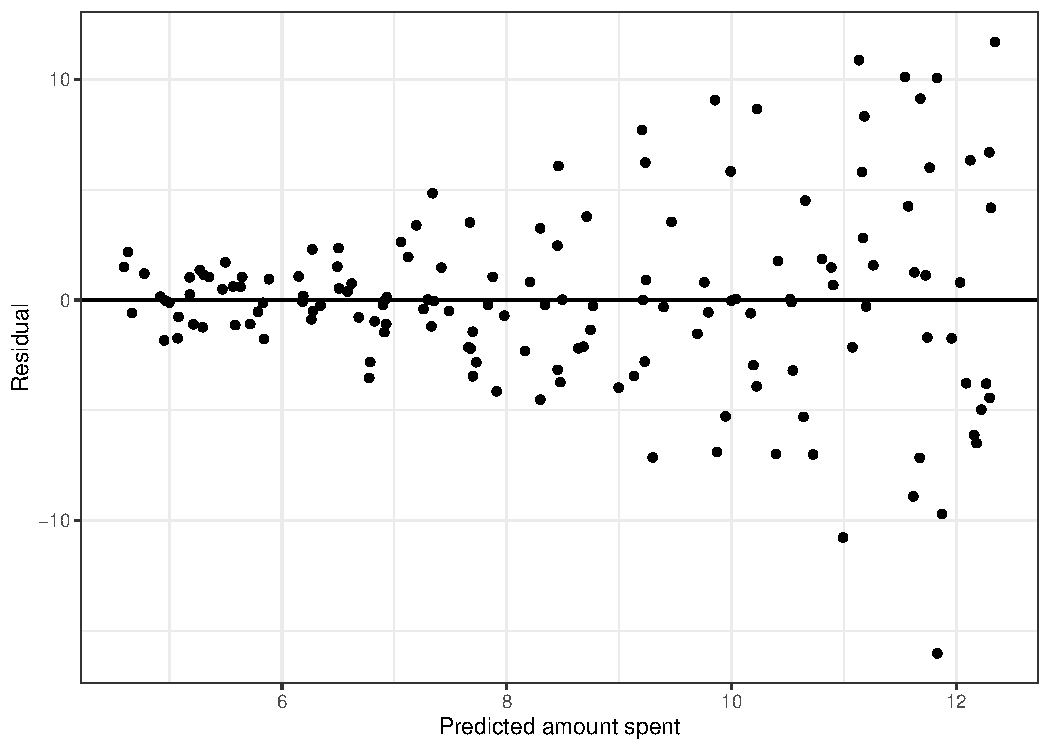
\includegraphics[scale=0.7]{residual_plot.pdf}
\end{center}


\rule{\textwidth}{1pt}

\item Which regression assumption is violated here? How does violation of that assumption affect our confidence interval?

\pagebreak

%%%%%%%%%%%%%%%%%%%%%%%%%%%%%%%%%%%%%%%%%%%%%

\item Your client looks at the residual plot and writes the following summary. ``The points are randomly scattered above and below the horizontal line, with no clear pattern to the residuals. Therefore, the independence and randomness assumptions are appropriate.'' Explain to your client why their summary incorrectly assesses the independence and randomness assumptions. Then correctly assess whether independence and randomness are reasonable for this data.

\vspace{8cm}

\item In order to check for outliers, what kind of plot would you need to make? Be clear about what information would be displayed on each axis, and which points in the plot you would call outliers. Give your answer in 1--3 sentences.

\pagebreak

%%%%%%%%%%%%%%%%%%%%%%%%%%%%%%%%%%%%%%%%


\huge{You are done!!! Whooo!!!}


%%%%%%%%%%%%%%%%%%%%%%%%%%%%%%%%%%%%%%%%


\end{enumerate}

%%%%%%%%%%%%%%%%%%%%%%%%%%%%

%\pagebreak

%\hdashrule[0.5ex]{\textwidth}{0.5pt}{3mm}
%\begin{center}
%\renewcommand{\arraystretch}{1.5}
%\begin{tabular}{| l | c | c | c | c | c | c  || c |}
%\hline
%				& 		& 		& 		& 		&	&  	&\\
%				& Q1-Q3		& Q4-6		& Q7		& Q8-Q10		 & Q11-Q12	 & Q13 & Total	\\
%\hline
%Points earned		& \textcolor{white}{xxxxx} &	\textcolor{white}{xxxxx}	& \textcolor{white}{xxxxx}	&	\textcolor{white}{xxxxx}&%\textcolor{white}{xxxxx}	&	\textcolor{white}{xxxxx} &	\textcolor{white}{xxxxx} \\
%\hline
%Available points	& 9 		& 12		& 9		& 9		&7 & 4 					& 50 \\
%\hline
%\end{tabular}

%\end{center}

\end{document}
